\documentclass[11pt,a4paper]{article}

\usepackage{graphicx}
\usepackage{listings}
\title{Semaphore using FreeRTOS on LPC2148}


\author{e-Yantra Team}
\date{\today}

\begin{document}
	\maketitle
	\newpage
	\tableofcontents
	\newpage
	
	
	\section{Introduction}
	There are a limited number of resources available to any system,Similarly any microcontroller has a limited number  resources available.
	\\ \\
	As the complexity of the application Increases the number of Tasks running also Increases,more and more Tasks compete for the available Processor time or The I/O devices available.
	\\ \\
	To ensure equal availability of resources to all the Tasks Operating Systems provide a facilities through semaphores.
	\\ 
	The Greek word sema means sign or signal, and -phore means carrier . So Semaphore = signalling.
	\\
	Semaphores can be classified into
	\\ 
	\begin{itemize}
	\item Binary Semaphores
	\item Mutex	 
	\item Counting Semaphores
	
	
	\end{itemize}
	\subsection{Binary Semaphores}
	
	Binary semaphores are used for Task synchronisation.
	If a process ocuppies a resource the value of Binary semaphore is 1 else 0 i.e it gives information only if the resource is available or not.
	
	\subsection{Mutex}
	
	Mutex stands for Mutual Exclusion.Any Task which requires a resource can "Block" the resource.when the Task uses the resource it can "Give" the resource.
	
	\subsection{Counting Semaphore}
	
	Counting semaphores are used to count resources and keep track of Multiple resources.
	\\
	\newpage 
	\subsection{Mutex vs Binary Semaphore}
	\begin{itemize}
		\item Mutexes are used for Resource Protection from other tasks//processes whereas Binary semaphores are used for task synchronistaion
		\\
		\item It is the responisibility of the occupying function to release the mutex,but a binary semaphore can be released even from ISR or any other functions.
		\\
		\item On the implementation level it is the Responibility of the Coder to ensure that the Mutex is only given by the task which takes it.
		
	\end{itemize}
		
	\section{Requirement}
	\begin{enumerate}
		\item Knowledge of C++ 
		\item FreeRTOS source files/API
		\item Keil compiler
		\item Flash magic
		\item FireBird V (LPC2148)
	\end{enumerate}
	
	
	
	
	\newpage	
	\section{Binary Semaphore}
	
\subsection{Code : }
	\lstinputlisting[language=c]{bin.c.}	
	\newpage
\subsection{Explanation}
	\begin{itemize}
	\item \textbf{Variable declaration}	
	
	\begin{lstlisting}
	SemaphoreHandle_t xSemaphore;
	\end{lstlisting}
	
	 This statement declares a variable of type "SemaphoreHandle\_t"
	
	\item \textbf{Creation of the semaphore}
	
	\begin{lstlisting}
	xSemaphore=xSemaphoreCreateBinary( );
	\end{lstlisting}

\item \textbf{Working of code}
	  \\
	  \\
	  The forward function Waits for portMAX\_DELAY i.e for maximum amount of time so that the control of Resources is available.
	  \\
	  \\
	  Similarly the back function waits for maximum time to get access to the resources.
	  \\
	  \\	
	  As soon as execution of Tasks starts the resources are occupied by the back function(vTaskDelay restricts forward function),The control\_switcher function is suspended for 1200 clock counts and Gives away the semaphore.
	  \\
	  \\
	  As soon as the semaphore is released the forward function waiting for allocation of resources occupies them,the cycle continues with control\_switcher releasing the semaphore.  
		\\
		\\
		\\
\item \textbf{Serial monitor Output} 
\\
\\
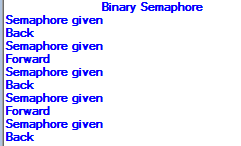
\includegraphics[width=10cm]{bin}

\end{itemize}
\newpage 
\section{Mutex}

\subsection{Code : }
\lstinputlisting[language=c]{mut.c.}	
\newpage

\subsection{Explanation}
\begin{itemize}
	\item \textbf{Variable declaration}	
	
	\begin{lstlisting}
	SemaphoreHandle_t xSemaphore;
	\end{lstlisting}
	
	This statement declares a variable of type "SemaphoreHandle\_t"
	
	\item \textbf{Creation of Mutex}
	
	\begin{lstlisting}
	xSemaphore = xSemaphoreCreateMutex();
	\end{lstlisting}
	
	\item \textbf{Working of code}
	\\
	\\
	There are Two Tasks forward and back, when executed
	\\
	\\
	The forward function Waits for 1000 clock cycles for the resources,In case the resources are not available the Task sends a message about The lack of availability of resources.
		Similarly the back function waits for same amount of time for resources.
	\\
	\\	
	As soon as execution of Tasks starts the resources are occupied by one of the the task and that task blocks the acess of those resources through a mutex.
	\\
	\\
The task executes and when the execution is completed it "Gives" the Mutex and therefore the releases the resources,another waiting task then occupies those resources and blocks for a period of time it requires.
	\\
	\\
	\\
	\item \textbf{Serial monitor Output} 
	\\
	\\
	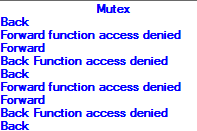
\includegraphics[width=8.5cm]{mut}
\end{itemize}

\newpage 

\section{Counting Semaphore Implemented by dining Philosophers Problem}

\subsection{Code : }
\lstinputlisting[language=c]{cont.c.}	
\newpage

\subsection{Explanation}
\begin{itemize}
	\item \textbf{Variable declaration}	
	
	\begin{lstlisting}
	SemaphoreHandle_t xSemaphore;
	\end{lstlisting}
	
	This statement declares a variable of type "SemaphoreHandle\_t"
	
	\item \textbf{Creation of Counting semaphore}
	
	\begin{lstlisting}
xSemaphore = xSemaphoreCreateCounting( 5, 5 );
	\end{lstlisting}
	
	Here 1st parameter gives the maximum count and 2nd parameter is the initial count.
	If the semaphore is used for counting events 2nd parameter would be 0 and if used for resources management it would be equal to maximum or initial count.
	\\
	\item \textbf{Task Creation }
	\begin{lstlisting}
	xTaskCreate(vfork,"Philospher 1", 300 ,"P1",
	 tskIDLE_PRIORITY + 1, NULL);
	.
	.
	\end{lstlisting}
	Here vfork is a single Task which on variation of Parameter P1,P2...etc behaves as a different task,ecah task has its own stack and act as if they are independent.All the tasks have same priority and get equal time at the processor.
	\\
	\item \textbf{Working of code}
	
	The Tasks created are by changing the parameters of a single task.
	\\
	\\
	When each time a "Philosopher" is allocated the processor time it checks for the number of available "Forks".If the forks are available and then check for the Right fork and the philosopher "picks up the left fork" then when the "Philosopher" again gains the processor time it waits for Left fork to be available and proceeds to eat.
	
	when 5 "Philosophers" are allocated simulatenously the semaphore keeps track of the available forks .
	
	
	\newpage
	\item \textbf{Serial monitor output}
	\\
	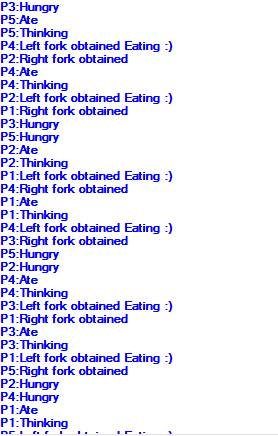
\includegraphics[width=12cm]{cont}
\end{itemize}
\newpage



	
	\section{References}
	\begin{enumerate}
	\item  http://www.rtos.be/2013/05/mutexes-and-semaphores-two-concepts-for-two-different-use-cases/
	
	\item http://www.ocfreaks.com/cat/embedded/lpc2148-tutorials/
	\item http://www.freertos.org/Inter-Task-Communication.html
	\item http://tinymicros.com/
	\item http://www.profdong.com/elc4438\_spring2016/\\USINGTHEFREERTOSREALTIMEKERNEL.pdf
	\end{enumerate}	
	\end{document}


